\documentclass[11pt,a4paper]{article}
\usepackage[utf8]{inputenc}
\usepackage[T1]{fontenc}
\usepackage{amsmath}
\usepackage{amsfonts}
\usepackage{amssymb}
\usepackage{graphicx}
\usepackage{tikz}
\usepackage{algorithm}
\usepackage{algorithmic}
\usepackage{listings}
\usepackage{xcolor}
\usepackage{geometry}
\usepackage{fancyhdr}
\usepackage{hyperref}
\usepackage{natbib}
\usepackage{amssymb}
\usepackage{pifont}

% Define checkmark and cross symbols
\newcommand{\cmark}{\ding{51}}
\newcommand{\xmark}{\ding{55}}

\geometry{margin=1in}
\pagestyle{fancy}
\fancyhf{}
\rhead{OBINexus Computing}
\lhead{Cryptographic Interoperability Standard v1.0}
\cfoot{\thepage}

% Define colors for code listings
\definecolor{codegreen}{rgb}{0,0.6,0}
\definecolor{codegray}{rgb}{0.5,0.5,0.5}
\definecolor{codepurple}{rgb}{0.58,0,0.82}
\definecolor{backcolour}{rgb}{0.95,0.95,0.92}

% Code listing style
\lstdefinestyle{mystyle}{
    backgroundcolor=\color{backcolour},   
    commentstyle=\color{codegreen},
    keywordstyle=\color{magenta},
    numberstyle=\tiny\color{codegray},
    stringstyle=\color{codepurple},
    basicstyle=\ttfamily\footnotesize,
    breakatwhitespace=false,         
    breaklines=true,                 
    captionpos=b,                    
    keepspaces=true,                 
    numbers=left,                    
    numbersep=5pt,                  
    showspaces=false,                
    showstringspaces=false,
    showtabs=false,                  
    tabsize=2
}
\lstset{style=mystyle}

\title{
    \textbf{OBINexus Cryptographic Interoperability and\\
    Pattern Normalization Standard v1.0}\\
    \large A Formal Specification for Regex-Based Primitive Matching\\
    and Isomorphic Reduction in Distributed Cryptographic Systems
}

\author{
    Nnamdi Michael Okpala\\
    \textit{OBINexus Computing}\\
    \texttt{obinexus.org}
}

\date{\today}

\begin{document}

\maketitle

\begin{abstract}
This document establishes the formal specification for cryptographic primitive interoperability within OBINexus computing infrastructure. The standard defines regex-based pattern matching for primitive identification, isomorphic reduction principles for canonical state normalization, and cross-language compatibility requirements. By treating cryptographic primitives as finite automaton states with regex fingerprints, this specification ensures deterministic behavior across heterogeneous environments while preventing encoding-based exploit vectors. The framework implements structural equivalence detection that operates across all levels of the Chomsky hierarchy, providing both computational efficiency and robust security properties for distributed cryptographic operations.
\end{abstract}

\tableofcontents
\newpage

\section{Introduction}

Modern cryptographic systems face increasing complexity in managing diverse primitive representations across programming languages, encoding schemes, and system architectures. Traditional approaches treat each primitive variant as a distinct computational problem, leading to bloated parsers, increased attack surfaces, and significant maintenance overhead.

The OBINexus Cryptographic Interoperability Standard addresses these challenges through a unified framework based on regular expression pattern matching and isomorphic reduction principles. This specification defines how cryptographic primitives are identified, validated, and normalized across all OBINexus infrastructure components.

\subsection{Scope and Applicability}

This standard applies to all OBINexus cryptographic operations, including but not limited to:
\begin{itemize}
    \item Key derivation and management systems
    \item Digital signature verification protocols
    \item Encrypted storage and transmission mechanisms
    \item Authentication and authorization frameworks
    \item Audit logging and compliance systems
\end{itemize}

\subsection{Design Principles}

The standard is built upon three fundamental principles derived from cryptographic theory \cite{okpala2025principles}:

\begin{enumerate}
    \item \textbf{Hardness}: Ensuring problems are easy to verify but hard to solve without knowledge
    \item \textbf{Completeness}: Guaranteeing the system can detect anomalies without relying on external assumptions
    \item \textbf{Soundness}: Ensuring inputs are only accepted from verified sources, preventing manipulation by randomness or guesswork
\end{enumerate}

\section{Pattern Matching and Identification}

\subsection{Regex Pattern Enforcement Policy}

All cryptographic primitive identification within OBINexus systems SHALL use deterministic regular expression patterns. The enforcement policy implements mandatory control logic for primitive validation:

\begin{lstlisting}[language=Python, caption=Mandatory Pattern Enforcement Logic]
def enforce_primitive_pattern(primitive_digest: str, 
                            context: str) -> ValidationResult:
    """
    Mandatory pattern enforcement for cryptographic primitives.
    MUST implement if/else control logic as specified.
    """
    # Phase 1: Pattern Recognition
    matched_patterns = []
    for pattern_state in REGISTERED_PATTERNS:
        if pattern_state.matches(primitive_digest):
            matched_patterns.append(pattern_state)
    
    # Phase 2: Collision Resolution (if multiple matches)
    if len(matched_patterns) == 0:
        return ValidationResult.REJECT_UNKNOWN_PATTERN
    elif len(matched_patterns) == 1:
        return ValidationResult.ACCEPT_SINGLE_MATCH
    else:
        # Longest pattern wins (most specific)
        canonical_pattern = max(matched_patterns, 
                              key=lambda p: len(p.pattern))
        return ValidationResult.ACCEPT_CANONICAL_RESOLUTION
    
    # Phase 3: Security Level Validation
    if canonical_pattern.security_level == "deprecated":
        if context in LEGACY_ALLOWED_CONTEXTS:
            return ValidationResult.ACCEPT_LEGACY_CONTEXT
        else:
            return ValidationResult.REJECT_DEPRECATED_SECURITY
    
    return ValidationResult.ACCEPT_VALIDATED
\end{lstlisting}

\subsection{Pattern Registration Format}

Cryptographic primitive patterns MUST conform to the following format specification:

\begin{center}
\texttt{<ALGORITHM>-<KEYSIZE>:[<HEX\_PATTERN>]\{<LENGTH>\}}
\end{center}

Examples of valid pattern registrations:
\begin{itemize}
    \item \texttt{RSA-2048:[a-f0-9]\{512\}} - RSA 2048-bit key with 512-character hex digest
    \item \texttt{AES-256:[a-f0-9]\{64\}} - AES 256-bit key with 64-character hex digest
    \item \texttt{ECDSA-P256:[a-f0-9]\{128\}} - ECDSA P-256 curve with 128-character hex digest
\end{itemize}

\section{Primitive Lifecycle and Policy}

\subsection{Version Evolution Model}

The primitive lifecycle implements non-destructive version evolution where new cryptographic standards register additional patterns without invalidating existing implementations. This approach ensures backward compatibility while enabling controlled security upgrades.

\begin{figure}[h]
\centering
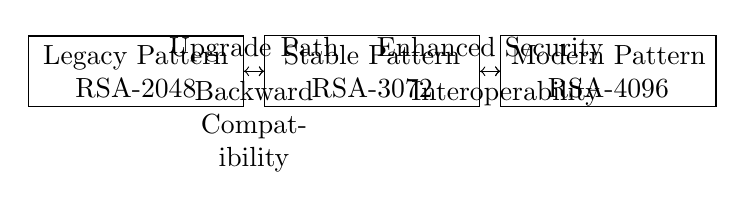
\begin{tikzpicture}[node distance=2cm, auto]
    \node (legacy) [rectangle, draw, text width=2.5cm, text centered] {Legacy Pattern\\RSA-2048};
    \node (stable) [rectangle, draw, text width=2.5cm, text centered, right of=legacy, xshift=1cm] {Stable Pattern\\RSA-3072};
    \node (modern) [rectangle, draw, text width=2.5cm, text centered, right of=stable, xshift=1cm] {Modern Pattern\\RSA-4096};
    
    \draw [->] (legacy) -- node {Upgrade Path} (stable);
    \draw [->] (stable) -- node {Enhanced Security} (modern);
    \draw [<->] (legacy) -- node [below, text width=2cm, text centered] {Backward Compatibility} (stable);
    \draw [<->] (stable) -- node [below, text width=2cm, text centered] {Interoperability} (modern);
\end{tikzpicture}
\caption{Primitive Version Evolution with Backward Compatibility}
\end{figure}

\subsection{Pattern Compatibility Matrix}

The compatibility matrix defines which primitive versions can interoperate:

\begin{table}[h]
\centering
\begin{tabular}{|l|c|c|c|c|}
\hline
\textbf{Algorithm} & \textbf{Legacy} & \textbf{Stable} & \textbf{Modern} & \textbf{Experimental} \\
\hline
RSA-2048 & \cmark & \cmark & \cmark & \xmark \\
RSA-3072 & \cmark & \cmark & \cmark & \cmark \\
RSA-4096 & \xmark & \cmark & \cmark & \cmark \\
AES-256 & \cmark & \cmark & \cmark & \cmark \\
ECDSA-P256 & \cmark & \cmark & \cmark & \xmark \\
ECDSA-P384 & \xmark & \cmark & \cmark & \cmark \\
\hline
\end{tabular}
\caption{Cryptographic Primitive Compatibility Matrix}
\end{table}

\section{Isomorphic Reduction Principle}

\subsection{Theoretical Foundation}

Building upon the Unicode-Only Structural Charset Normalizer framework \cite{okpala2025isomorphic}, this standard applies isomorphic reduction principles to cryptographic primitive normalization. The key insight is that structurally equivalent primitive representations should be treated as identical automaton states.

\textbf{Definition 1} (Cryptographic Isomorphic Reduction): Let $P_1$ and $P_2$ be primitive representations from different encoding schemes. Primitives $P_1$ and $P_2$ are isomorphically reducible if there exists a structure-preserving mapping $\phi : P_1 \rightarrow P_2$ such that:

$$\phi(P_1) \equiv P_2 \text{ (cryptographically equivalent)}$$

\textbf{Theorem 1} (Primitive Equivalence): For any set of cryptographic primitive encodings $E = \{e_1, e_2, \ldots, e_n\}$ representing the same cryptographic content, there exists a minimal canonical form $c$ such that:

$$\forall e_i \in E : \phi(e_i) = c$$

where $\phi$ is a normalization function preserving cryptographic equivalence.

\subsection{Automaton-Based Primitive Modeling}

Cryptographic primitive recognition is modeled as a finite state automaton problem where each encoding variant represents a distinct path through the automaton that leads to the same accepting state representing the canonical primitive.

\textbf{Definition 2} (Cryptographic Primitive Automaton): A Cryptographic Primitive Automaton (CPA) is defined as the 5-tuple:

$$A_{CP} = (Q, \Sigma, \delta, q_0, F)$$

where:
\begin{itemize}
    \item $Q$ is the finite set of primitive states
    \item $\Sigma$ is the input alphabet (including encoded primitive digests)
    \item $\delta : Q \times \Sigma \rightarrow Q$ is the transition function
    \item $q_0 \in Q$ is the initial state
    \item $F \subseteq Q$ is the set of accepting states representing validated primitives
\end{itemize}

\section{Canonical Mapping Functions}

\subsection{Pattern Normalization Algorithm}

The canonical mapping function implements structural equivalence detection across multiple primitive encoding schemes:

\begin{algorithm}
\caption{Cryptographic Primitive State Minimization}
\begin{algorithmic}[1]
\REQUIRE Set of primitive encodings $E$, Primitive Automaton $A_{CP}$
\ENSURE Minimized automaton $A_{min}$ with canonical mappings
\STATE Initialize equivalence classes: $C = \{F, Q \setminus F\}$
\STATE $changed \leftarrow true$
\WHILE{$changed$}
    \STATE $changed \leftarrow false$
    \FOR{each class $C_i \in C$}
        \STATE Initialize signature groups: $splits \leftarrow \emptyset$
        \FOR{each state $q \in C_i$}
            \STATE Compute transition signature: $signature(q) = \{(\sigma, class(\delta(q, \sigma))) | \sigma \in \Sigma\}$
            \STATE Add $q$ to $splits[signature(q)]$
        \ENDFOR
        \IF{$|splits| > 1$}
            \STATE Replace $C_i$ with $splits.values()$ in $C$
            \STATE $changed \leftarrow true$
        \ENDIF
    \ENDFOR
\ENDWHILE
\STATE Construct $A_{min}$ using equivalence classes as states
\RETURN $A_{min}$, canonical mapping for each encoding
\end{algorithmic}
\end{algorithm}

\subsection{Canonical Form Examples}

The following examples demonstrate canonical mapping for common primitive encoding variations:

\begin{lstlisting}[caption=Canonical Mapping Examples]
# RSA Key Encoding Variations -> Canonical Form
phi("rsa-2048:a1b2c3d4...") = "RSA-2048:A1B2C3D4..."
phi("RSA_2048:a1b2c3d4...") = "RSA-2048:A1B2C3D4..."
phi("rsa2048:a1b2c3d4...")  = "RSA-2048:A1B2C3D4..."

# AES Key Encoding Variations -> Canonical Form  
phi("aes-256:f1e2d3c4...")  = "AES-256:F1E2D3C4..."
phi("AES_256:f1e2d3c4...")  = "AES-256:F1E2D3C4..."
phi("aes256:f1e2d3c4...")   = "AES-256:F1E2D3C4..."

# Hash Digest Variations -> Canonical Form
phi("sha256:0x1a2b3c...")   = "SHA256:1A2B3C..."
phi("SHA-256:1a2b3c...")    = "SHA256:1A2B3C..."
phi("sha_256:1a2b3c...")    = "SHA256:1A2B3C..."
\end{lstlisting}

\section{Unicode Normalization and Regex Consistency}

\subsection{Cross-Language Deterministic Regex Subset}

To ensure consistent behavior across Python, Lua, and C implementations, this standard defines a restricted regex subset that provides deterministic matching across all supported languages:

\textbf{Allowed Regex Constructs:}
\begin{itemize}
    \item Character classes: \texttt{[a-f0-9]}, \texttt{[A-Z]}, \texttt{[0-9]}
    \item Quantifiers: \texttt{\{n\}}, \texttt{\{n,m\}}
    \item Anchors: \texttt{\^{}}, \texttt{\$}
    \item Literals: Alphanumeric characters and hyphens
\end{itemize}

\textbf{Prohibited Regex Constructs:}
\begin{itemize}
    \item Lookaheads and lookbehinds: \texttt{(?=...)}, \texttt{(?!...)}
    \item Non-greedy quantifiers: \texttt{*?}, \texttt{+?}
    \item Unicode categories: \texttt{\textbackslash p\{...\}}
    \item Word boundaries: \texttt{\textbackslash b}
\end{itemize}

\subsection{Unicode Character Normalization}

All primitive digest strings SHALL be normalized using the Unicode-Only Structural Charset Normalizer (USCN) approach before pattern matching. This eliminates encoding-based exploit vectors:

\begin{lstlisting}[caption=Unicode Normalization Implementation]
def normalize_primitive_input(input_string: str) -> str:
    """
    Apply USCN normalization to eliminate encoding variations.
    """
    # Phase 1: Decode common encoding variations
    normalized = input_string
    for encoding_variant, canonical in ENCODING_MAPPINGS.items():
        normalized = normalized.replace(encoding_variant, canonical)
    
    # Phase 2: Case normalization for hex strings
    if is_hex_string(normalized):
        normalized = normalized.upper()
    
    # Phase 3: Delimiter standardization
    normalized = standardize_delimiters(normalized)
    
    return normalized
\end{lstlisting}

\section{Security Guarantees}

\subsection{Exploit Vector Elimination}

The isomorphic reduction approach eliminates common cryptographic primitive exploit vectors by normalizing all inputs to canonical forms before validation.

\textbf{Proposition 1} (Security Invariant): For any primitive input string $s$ containing encoded characters, the OBINexus standard guarantees:

$$validate(normalize(s)) \equiv validate(canonical(s))$$

where validation occurs exclusively on the normalized canonical form, preventing encoding-based bypasses.

\subsection{Path Traversal Prevention for Primitive References}

Traditional primitive reference validation is vulnerable to encoding variations:

\begin{lstlisting}[caption=Vulnerable Primitive Reference Validation]
def vulnerable_primitive_check(primitive_ref: str) -> bool:
    # Fails for encoding variants
    if "../" in primitive_ref:
        return False  # Blocked
    return True

# These bypass the filter:
vulnerable_primitive_check("%2e%2e%2f")  # Returns True (BYPASS)
vulnerable_primitive_check("%c0%af")     # Returns True (BYPASS)
\end{lstlisting}

The OBINexus standard prevents these exploits through structural normalization:

\begin{lstlisting}[caption=Hardened Primitive Reference Validation]
def secure_primitive_check(primitive_ref: str) -> bool:
    # Normalizes ALL variants before validation
    canonical = normalize_primitive_input(primitive_ref)
    if "../" in canonical:
        return False  # Blocked
    return True

# All encoding variants are caught:
secure_primitive_check("%2e%2e%2f")  # Returns False (SECURE)
secure_primitive_check("%c0%af")     # Returns False (SECURE)
secure_primitive_check("../")        # Returns False (SECURE)
\end{lstlisting}

\section{Audit Trail and Logging Syntax}

\subsection{Secure Pattern Hash References}

To prevent information disclosure while maintaining audit integrity, all log entries SHALL reference cryptographic patterns using secure hash identifiers rather than exposing raw pattern strings.

\begin{lstlisting}[caption=Audit Trail Pattern Reference Implementation]
class SecureAuditNode:
    """Secure audit trail node for primitive operations."""
    
    def __init__(self, primitive_digest: str, pattern_state: State):
        self.timestamp = datetime.utcnow()
        self.primitive_hash = sha256(primitive_digest).hexdigest()[:16]
        self.pattern_hash = sha256(pattern_state.pattern).hexdigest()[:16]
        self.operation_context = get_current_context()
        # Never store raw primitive_digest or pattern in logs
    
    def to_audit_record(self) -> dict:
        return {
            "timestamp": self.timestamp.isoformat(),
            "primitive_ref": f"PRIM_{self.primitive_hash}",
            "pattern_ref": f"PAT_{self.pattern_hash}",
            "context": self.operation_context,
            "compliance_level": "OBINexus-v1.0"
        }
\end{lstlisting}

\subsection{Audit Trail Compliance Requirements}

All OBINexus cryptographic operations MUST generate audit records conforming to this specification:

\begin{table}[h]
\centering
\begin{tabular}{|l|l|l|}
\hline
\textbf{Field} & \textbf{Format} & \textbf{Description} \\
\hline
timestamp & ISO 8601 UTC & Operation execution time \\
primitive\_ref & PRIM\_[16-char hex] & Hashed primitive identifier \\
pattern\_ref & PAT\_[16-char hex] & Hashed pattern identifier \\
context & String & Operation context identifier \\
compliance\_level & OBINexus-v1.0 & Standard version compliance \\
\hline
\end{tabular}
\caption{Mandatory Audit Record Format}
\end{table}

\section{Formal Definitions}

\subsection{Regex Automaton Definition}

\textbf{Definition 3} (Regex Automaton): A Regex Automaton $AR$ for cryptographic primitive matching is a 5-tuple:

$$AR = (Q_R, \Sigma, \delta_R, q_0, F)$$

where each state $q \in Q_R$ is associated with a regular expression pattern $pattern(q)$ such that the automaton accepts input string $w$ if and only if $w$ matches $pattern(q_f)$ for some final state $q_f \in F$ reachable from $q_0$ via input $w$.

\subsection{Pattern Compatibility Matrix Definition}

\textbf{Definition 4} (Compatibility Matrix): The Pattern Compatibility Matrix $M$ is a function:

$$M: PatternSpace \times PatternSpace \rightarrow \{COMPATIBLE, INCOMPATIBLE, LEGACY\_ONLY\}$$

where $PatternSpace$ represents the set of all registered cryptographic primitive patterns.

\subsection{Canonical Transition Model}

\textbf{Definition 5} (Canonical Transition): A canonical transition is a mapping $T: State \times Input \rightarrow CanonicalState$ where multiple equivalent input encodings map to the same canonical state, ensuring deterministic behavior regardless of input encoding variation.

\section{Cross-Language Compatibility}

\subsection{Implementation Requirements}

All OBINexus cryptographic systems MUST implement pattern matching using the cross-language compatible regex subset defined in Section 5.1. Reference implementations SHALL be provided for:

\begin{itemize}
    \item Python 3.8+ using the \texttt{re} module
    \item Lua 5.4+ using POSIX-compatible patterns  
    \item C99+ using POSIX regex library (\texttt{regex.h})
\end{itemize}

\subsection{Validation Framework}

A cross-language validation framework ensures consistent behavior across all implementations:

\begin{lstlisting}[caption=Cross-Language Validation Test]
def validate_cross_language_consistency():
    """Validate pattern matching consistency across languages."""
    test_cases = [
        ("RSA-2048:A1B2C3...", "rsa-2048:a1b2c3..."),
        ("AES-256:F1E2D3...", "aes_256:f1e2d3..."),
        ("SHA256:1A2B3C...", "sha-256:1a2b3c...")
    ]
    
    for canonical, variant in test_cases:
        python_result = python_normalize(variant)
        lua_result = lua_normalize(variant) 
        c_result = c_normalize(variant)
        
        assert python_result == lua_result == c_result == canonical
        assert all_match_pattern(canonical, REGISTERED_PATTERNS)
\end{lstlisting}

\section{Compliance and Enforcement}

\subsection{Mandatory Implementation Requirements}

All systems claiming OBINexus v1.0 compatibility MUST:

\begin{enumerate}
    \item Implement the complete pattern enforcement policy (Section 2.1)
    \item Support primitive lifecycle management (Section 3)
    \item Apply isomorphic reduction normalization (Section 4)
    \item Use secure audit trail format (Section 6)
    \item Pass cross-language validation tests (Section 8.2)
\end{enumerate}

\subsection{Compliance Verification}

Compliance verification SHALL be performed using the OBINexus Cryptographic Test Suite, which validates:

\begin{itemize}
    \item Pattern matching determinism across supported languages
    \item Canonical mapping function correctness
    \item Security invariant preservation under encoding variations
    \item Audit trail format adherence
    \item Performance benchmarks for production deployment
\end{itemize}

\section{Conclusion}

The OBINexus Cryptographic Interoperability and Pattern Normalization Standard provides a mathematically rigorous foundation for cryptographic primitive identification and validation across heterogeneous computing environments. By applying isomorphic reduction principles and deterministic pattern matching, this standard eliminates common exploit vectors while ensuring backward compatibility and cross-language consistency.

As stated in the foundational OBINexus principle: "Structure is the final syntax" \cite{okpala2025isomorphic}. This standard embodies that philosophy by making structural equivalence the foundation for cryptographic security rather than surface-level pattern enumeration.

Implementation of this standard ensures that OBINexus cryptographic infrastructure operates with deterministic behavior, robust security properties, and comprehensive audit capabilities across all deployment environments.

\bibliographystyle{plain}
\begin{thebibliography}{9}

\bibitem{okpala2025principles}
Okpala, N.M. (2025).
\textit{Principles of Cryptography: Hardness, Completeness, and Soundness}.
OBINexus Computing Technical Documentation.

\bibitem{okpala2025isomorphic}
Okpala, N.M. (2025).
\textit{Unicode-Only Structural Charset Normalizer: Isomorphic Reduction as a Feature, Not a Bug}.
OBINexus Computing.

\bibitem{okpala2025cryptographic}
Okpala, N.M. (2025).
\textit{Building the Future of Encryption - A Proposal for Standardised Cryptographic Primitives}.
OBINexus Medium Publication.

\bibitem{chomsky1956}
Chomsky, N. (1956).
\textit{Three models for the description of language}.
IRE Transactions on Information Theory, 2(3), 113-124.

\bibitem{myhill1957}
Myhill, J. (1957).
\textit{Finite automata and their decision problems}.
IBM Journal of Research and Development, 1(1), 4-14.

\bibitem{nerode1958}
Nerode, A. (1958).
\textit{Linear automaton transformations}.
Proceedings of the American Mathematical Society, 9(4), 541-544.

\end{thebibliography}

\end{document}